\documentclass[10pt,a4paper]{article}
\usepackage[latin1]{inputenc}
\usepackage{amsmath}
\usepackage{amsfonts}
\usepackage{amssymb}
\usepackage{amsthm}
\usepackage{mathtools}
\usepackage{bm}
\usepackage{standalone}
\usepackage{graphicx}
\usepackage{float}
\usepackage{gensymb}
% Use \bm{x} for vectors/matrices in bold AND italic

\newcommand{\vectornorm}[1]{\left\|#1\right\|}

\begin{document}
\title{Programming project in TMA4220 \\ Part 2B \\ Helmholtz' Equation For Electromagnetic Waves}
\author{Anders Opskar Voldsund \\ Andreas Borgen Longva \\ Espen Johansen Velsvik}
\maketitle

\theoremstyle{definition}
\newtheorem{definition}{Definition}

\newtheorem{theorem}{Theorem}[section]
\newtheorem{corollary}{Corollary}[theorem]
\newtheorem{lemma}[theorem]{Lemma}
\newtheorem{algorithm}{Algorithm}


\documentclass[10pt,a4paper]{article}
\usepackage[latin1]{inputenc}
\usepackage{amsmath}
\usepackage{amsfonts}
\usepackage{amssymb}
\begin{document}

\section*{Introduction}
The Helmholtz equation,
\begin{equation}
\begin{aligned}
\label{Helmholtz}
\Delta \psi + k^2 \psi = g,
\end{aligned}
\end{equation}
is a time-independent form of the wave equations which often arise in physical problems involving the computation of electromagnetic radiation. In the modeling of electromagnetic waves $\psi$ represents the Fourier transform of either the electric field $E$ or the magnetic field $H$. $k$ is called the wavenumber, and from the derivation of the Helmholtz' equation from Maxwell's equations in vacuum it is seen that $k = \frac{2\pi f}{c}$. Here $f$ is the frequency of the electromagnetic waves and $c = \frac{1}{\sqrt{\mu_0 \epsilon_0}}$ is the speed of light, where $\mu_0$ and $\epsilon_0$ are the permeability and permittivity in vacuum.

\end{document}

\documentclass[10pt,a4paper]{article}
\usepackage[latin1]{inputenc}
\usepackage{amsmath}
\usepackage{amsfonts}
\usepackage{amssymb}
\begin{document}

\section*{The Weak Formulation}
We consider the following Dirichlet problem:
\begin{equation}
\begin{aligned}
\label{Helmholtz_Dir}
\Delta \psi + k^2 \psi &= g  \quad \text{in} \, \Omega \\
\psi &= 0 \quad \text{on} \, \partial \Omega.
\end{aligned}
\end{equation}
To derive a weak formulation the equation is multiplied with a suiting test function $v \in X $ and integrated over the domain $\Omega$. The left hand side gives:
\begin{align*}
\int_\Omega \nabla \psi v &+ k^2 \psi v \, \mathrm{d} \Omega \\
&\Downarrow \\
\int_{\partial \Omega} \frac{\partial \psi}{\partial n} v \, \mathrm{d} \Omega + \int_\Omega & k^2 \psi v - \nabla \psi \nabla v \, \mathrm{d} \Omega.
\end{align*}
At this point we can make a choice for the space of $v$. We choose $v$ to lie in the following space:
\begin{align*}
X = H^1_0(\Omega) = \left\{ v \in H^1(\Omega) : v = 0 \text{ on }   \partial \Omega \right\},
\end{align*}
where
\begin{align*}
H^1(\Omega) = \left\{ v: \Omega \rightarrow \mathbb{R}: v \in L^2(\Omega), v' \in L^2(\Omega) \right\}.
\end{align*}
Since $v$ disappears on the boundary we are left with the following expression:
\begin{align*}
\int_\Omega & k^2 \psi v - \nabla \psi \nabla v \, \mathrm{d} \Omega = \int_\Omega gv \, \mathrm{d} \Omega.
\end{align*}
Let now $a(u,v)$ and $F(v)$ be defined as the following functionals:
\begin{align*}
a(u,v) &= \int_\Omega  \nabla u \nabla v - k^2 u v  \, \mathrm{d} \Omega  \quad \text{and} \\
F(v) &= - \int_\Omega gv \, \mathrm{d} \Omega.
\end{align*}
This implies that $a(u,v) = F(v)$. The following problem is called the weak formulation of (\ref{Helmholtz_Dir}):
\begin{equation}
\begin{aligned}
\label{Helmholtz_weak}
\text{find} \, u \in H^1_0(\Omega): \quad a(u,v) = F(v) \quad \forall \, v \in H^1_0(\Omega).
\end{aligned}
\end{equation}
The functional $a(u,v)$ is continuous. This is seen by the following, where we have used the Poincaré inequality $\vectornorm{u}_{L^2} \leq C |u|_{H^1}$ for positive $C$, with the latter denoting the seminorm.
\begin{align*}
|a(u,v)| &= |\int_\Omega  \nabla u \nabla v - k^2 u v \, \mathrm{d} \Omega| \\
 		& \leq |\int_\Omega \nabla u \nabla v \, \mathrm{d} \Omega| + k^2 |\int_\Omega u v \, \mathrm{d} \Omega| \\
 		\text{Cauchy-Schwarz} \quad & \leq \vectornorm{\nabla u}_{L^2(\Omega)} \vectornorm{\nabla v}_{L^2(\Omega)} + k^2 \vectornorm{u}_{L^2(\Omega)} \vectornorm{v}_{L^2(\Omega)} \\
		& = |u|_{H^1(\Omega)} |v|_{H^1(\Omega)} + k^2 \vectornorm{u}_{L^2(\Omega)} \vectornorm{v}_{L^2(\Omega)} \\
		\text{Poincaré} \quad & \leq |u|_{H^1(\Omega)} |v|_{H^1(\Omega)} + k^2 C_1 |{u}|_{H^1(\Omega)} |{v}|_{H^1(\Omega)} \\
		& = (1 + C_1 k^2) |u|_{H^1(\Omega)} |v|_{H^1(\Omega)} \\
		& \leq (1 + C_1 k^2) C_2 \vectornorm{u}_{H^1(\Omega)} \vectornorm{v}_{H^1(\Omega)} \\
		&= M \vectornorm{u}_{H^1(\Omega)} \vectornorm{v}_{H^1(\Omega)},
\end{align*}

where we have used the equivalence of the $H^1$ norm and semi-norm (property 2.5 in Quarteroni \cite{Quarteroni}).
The functional $a(u,v)$ is also coercive under certain conditions, since
\begin{align*}
a(u,u) &= \int_\Omega  \nabla u \nabla u - k^2 u u \, \mathrm{d} \Omega \\
 		& = \int_\Omega  |\nabla u|^2 \, \mathrm{d} \Omega - \int_{\Omega} k^2 |u|^2 \, \mathrm{d} \Omega \\
 		& =  \vectornorm{\nabla u}_{L^2(\Omega)}^2 - k^2 \vectornorm{u}_{L^2(\Omega)}^2\\
\text{Poincaré} \quad & \geq |u|^2_{H^1(\Omega)} - k^2 C_p^2 |u|^2_{H^1(\Omega)} \\
		& = (1 - k^2 C_p^2) |u|^2_{H^1(\Omega)} \\
		& \geq (1 - k^2 C_p^2) C \vectornorm{u}^2_{H^1(\Omega)} \\
		& = \alpha \vectornorm{u}^2_{H^1(\Omega)}.
\end{align*}

Here we have once again used the equivalence of the norm and semi-norm. Lastly the functional is bilinear, since it is linear in each component. The bilinear functional $F(v)$ is continuous:
\begin{align*}
|F(v)| &= |\int_\Omega gv \, \mathrm{d} \Omega| \leq \vectornorm{g}_{L^2(\Omega)} \vectornorm{v}_{L^2(\Omega)} \\
       &= M \vectornorm{v}_{L^2(\Omega)},
\end{align*}
and from the Lax-Milgram theorem there exists a unique solution to (\ref{Helmholtz_weak}) when $k^2 \leq \frac{1}{C_p^2}$ where $C_p$ is a Poincaré constant.

\end{document}

\documentclass[10pt,a4paper]{article}
\usepackage[latin1]{inputenc}
\usepackage{amsmath}
\usepackage{amsfonts}
\usepackage{amssymb}
\begin{document}


\section*{Relation to The Wave Equation}
As already stated, the Helmholtz equation for the modeling of electromagnetic waves can be derived from the Maxwell's equations in vacuum
\begin{align*}
\nabla \times E &= - \frac{\partial H}{\partial t} \\
\nabla \times H &= \mu_0 \epsilon _0 \frac{\partial E}{\partial t} \\
\nabla \cdot E &= 0 \\
\nabla \cdot H &= 0
\end{align*}

where $E: \Omega \times \mathbb{R}_+ \rightarrow \mathbb{R}^3$ is the electric field and $H: \Omega \times \mathbb{R}_+ \rightarrow \mathbb{R}^3$ is the magnetic field. It can be shown (\cite{Project}) that the equations can be decoupled into the wave equation for each component of the electric and magnetic field,
\begin{equation}
\begin{aligned}
\label{Wave}
\frac{\partial^2 \phi}{\partial t^2} - c^2 \Delta \phi = 0, 
\end{aligned}
\end{equation}
where $\phi$ is a spatial component for $E$ or $H$. To arrive at the Helmholtz equation we take the Fourier transform of $\phi$. From \cite{Helmholtz-Wave} we have that if $u(x,t) = \psi (x)e^{-i \omega t}$ satisfies (\ref{Wave}), then $\psi (x)$ is a solution to (\ref{Helmholtz}). This means that by numerically solving the Helmholtz equation, we are modeling the amplitude of the wave for one of the spatial components of the two fields $E$ and $H$.

\end{document}

\documentclass[10pt,a4paper]{article}
\usepackage[latin1]{inputenc}
\usepackage{amsmath}
\usepackage{amsfonts}
\usepackage{amssymb}
\usepackage{mathtools}
\usepackage{bm}
\usepackage{standalone}
\usepackage{graphicx}
\usepackage{float}
\begin{document}

\section*{Mesh Generation}
One of the major strengths of the finite element method is its ability to break down a problem on a global domain to a problem on individual, simpler elements that together constitute an approximation of the domain. As the complexity of the geometry of the problem domain increases, the need for automatic and reliable meshing procedures is evident. 

\begin{figure}[htb]
	\centering
    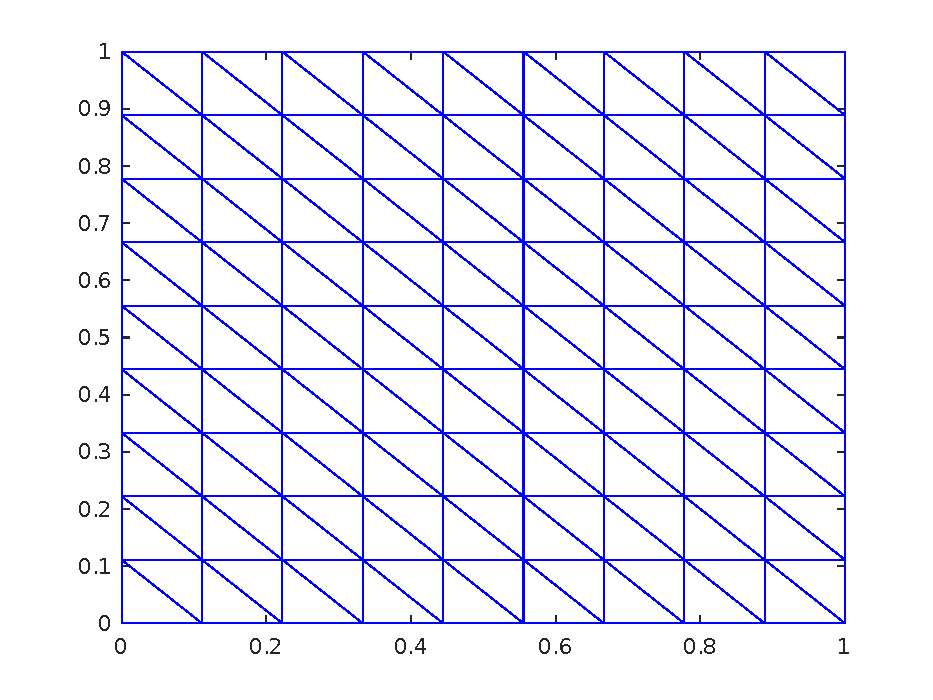
\includegraphics[width=0.9\textwidth]{figures/basic_rect_mesh}
    \caption{A very basic meshing procedure for trivial geometries. Simply perform a Delaunay triangulation on a regular grid of points.}
    \label{fig:basic_rect_mesh}
\end{figure}

Figure \ref{fig:basic_rect_mesh} illustrates a first attempt at a basic meshing procedure. Given a very simple domain, a regular grid of points are triangulated using Delaunay triangulation. This approach has some very obvious limitations. For one, it is not immediately clear how to deal with unions of geometric shapes which may exhibit local properties, such as density or electrical permittivity. Simply overlaying the geometries on top of the grid is likely to result in very ill-shaped triangles, which may be disastrous for convergence of the finite element method. From these observations we may formulate some goals for practical mesh algorithms:

\begin{itemize}
  \item Preserve boundaries of original geometries.
  \item Propagate local properties of geometry to elements in mesh.
  \item Generate meshes with well-shaped elements.
  \item Generate meshes with the minimum number of elements to adequately capture the geometry.
\end{itemize}

The last point is not of crucial importance for our work, but in many cases it is desirable to only generate triangles where needed, and instead take advantage of adaptive mesh refinement to constrain dense regions of mesh elements to parts of the domain where they are needed.

The Swiss army knife of mesh generation is the Delaunay triangulation. Given a set of points, it generates a triangulation of the convex hull of the points, with the property that no points are contained inside the circumcircle of any triangle. Note that for the purposes of this project, we are only concerned with 2D meshes. A useful extension is the Constrained Delaunay Triangulation, which is similar to Delaunay triangulation, but imposes constraints on which vertices in the triangulation must be connected by edges. A constrained Delaunay triangulation does not in general have the Delaunay property.

Since it's generally harder to reduce a fine mesh to a coarse mesh, most mesh generation algorithms iteratively refine a coarse starting mesh until certain quality metrics are fulfilled. This might for instance be a minimum angle or maximum edge length. While there are many approaches to mesh refinement, we have mainly looked at a variant of Ruppert's algorithm \cite{ruppert}. In particular, Shewchuk \cite{shewchuk} demonstrates that it can be formulated with a Constrained Delaunay Triangulation as input. The aforementioned papers demonstrate the algorithm in detail, so we will only discuss the main points. As Shewchuk points out, a very interesting feature of Ruppert's algorithm is that while it takes a constrained Delaunay triangulation as input, its output is in fact Delaunay. Essentially, the output of the algorithm has two crucial properties: it is Delaunay, which minimizes the minimum angle of the triangles, and the triangles have a certain quality given constraints on size and shape.

\subsection*{Ruppert's algorithm}
In the following, a \emph{segment} is a constrained edge in the input constrained Delaunay triangulation, and every segment consists of a set of \emph{subsegments} in the iteratively refined triangulation. Note in particular that the set of subsegments is a subset of the set of edges in the triangulation, and that every segment is also a subsegment. Recall also that the \emph{circumcenter} of a triangle is the center of the unique circle such that all three vertices of the triangle lie exactly on the circle boundary.

\theoremstyle{definition}
\begin{definition}{\textbf{Encroached subsegment}}
A subsegment is \emph{encroached} if a vertex of the triangulation is contained in its \emph{diametral circle}, which is the smallest circle that contains the subsegment.
\end{definition}

\begin{figure}[htb]
	\centering
    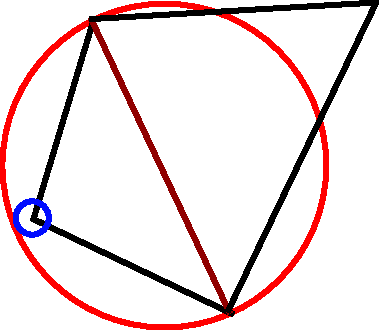
\includegraphics[width=0.6\textwidth]{figures/encroached}
    \caption{An example of an encroached subsegment. The dark red edge is a subsegment, the red circle its diametral circle and the vertex enclosed in the blue circle is a vertex that encroaches upon the subsegment.}
    \label{fig:encroached}
\end{figure}

It turns out that a constrained Delaunay triangulation without encroached subsegments is in fact Delaunay \cite{shewchuk}. Given the two output goals of Delaunay and triangle quality, the main idea of Ruppert's algorithm is to iteratively split any encroached subsegments until none remain, before it attempts to insert the circumcenters of ill-shaped triangles into the triangulation.

Figure \ref{fig:encroached} illustrates an encroached subsegment. A coarse outline of the algorithm follows. Note that when a point is inserted into the triangulation, an incremental Delaunay refinement algorithm is performed locally to compute the resulting triangulation.

\begin{algorithm}{\textbf{Ruppert's algorithm} (outline)}
\begin{enumerate}
	\item For any encroached subsegment, insert a vertex on its midpoint into the 	triangulation, effectively splitting the subsegment into two subsegments.
	\item Repeat the previous step until no subsegments are encroached.
	\item Consider a single poorly shaped triangle. If its circumcenter encroaches upon any subsegments, split the subsegments. Otherwise, insert the circumcenter into the triangulation.
	\item Repeat the algorithm from step 1 until there are no encroached edges and no poorly shaped triangles.
\end{enumerate}
\end{algorithm}

In \cite{ruppert}, Ruppert proves that given certain bounds on the angles of the input constraints, the algorithm terminates for a maximum angle of $20 \degree$, though he notes that in practice you are able to select larger values up to $\approx 30 \degree$. In \cite{shewchuk} it is claimed that the angles of the constrained segments in the input graph must be larger than $60 \degree$ to guarantee termination.

For practical purposes, such bounds on the input are not realistic, and so practical implementations must guarantee termination in the face of badly shaped input data. Some practical algorithms for deciding when to terminate are found in \cite{shewchuk}. A more recent and arguably better approach was introduced by Miller-Pav-Walkington in \cite{miller}.

\subsection*{Mesh generation implementation}
\subsubsection*{Ruppert's from scratch}
We implemented a version of Ruppert's algorithm in MATLAB using MATLAB's builtin Delaunay triangulation methods. In particular, MATLAB offers us a black box procedure for iterative Delaunay triangulation, so while it is convenient for on-the-fly inserting points as we are iterating, it does not give us any information about which triangles have changed after each change, so we must scan the entire set of triangles to determine what changed upon every iteration. This results in a rather disastrous time-complexity for our implementation.
Hence, while our implementation generates nice meshes for relatively small triangulations, and is capable of handling relatively general geometries (assuming angles are not too sharp), it simply does not terminate in reasonable time for finer meshes. Due to time and space constraints, we've omitted runtime and complexity evaluations of our implementation. 

Since the only way to remedy this is to implement the incremental Delaunay algorithm from scratch, we decided to instead look for existing stable, mature and faster mesh refinement implementations.

\subsubsection*{MATLAB PDE Toolbox}
The MATLAB PDE Toolbox contains a set of functions which are able to generate and refine meshes for almost arbitrary geometries. It is however rather inconvenient to use from the command-line, so we wrapped its functionality in a simple to use interface, allowing us to easily build relatively complicated geometries with different materials.

Although the meshing algorithm is much faster than our own custom implementation, it evidently still suffers from a relatively high time-complexity, as we were still unable to generate meshes of the desired resolution. Hence in practice we sometimes lowered the frequency of the modelled signal.

\end{document}

\documentclass[10pt,a4paper]{article}
\usepackage[latin1]{inputenc}
\usepackage{amsmath}
\usepackage{amsfonts}
\usepackage{amssymb}
\begin{document}

\section*{Introducing Spatially Varying Wave Number}
By introducing a spatially varying wave number given by
\begin{align}\label{eq:spatialWaveNumber}
k(x) = \frac{\omega}{c(x)} = \frac{\omega}{\sqrt{\mu(x)\epsilon(x)}},
\end{align}
we are able to model a more realistic scenario for how the signal will behave in our domain. In our implementation we can create geometric shapes where all triangles enclosed in this shape will be of the same material. Each material has a different wave number calculated from the material's permeability $\mu$ and permittivity $\epsilon$, as given in \eqref{eq:spatialWaveNumber}.

In our final example, we have modeled a rectangular house with wooden walls, a circular pool with water, and a rectangular box with walls made of lead. The rest of the domain contains air. As the $k$-value will vary for each of the materials, we see that the signal behaves differently in regions of different materials.





\end{document}

\documentclass[10pt,a4paper]{article}
\usepackage[latin1]{inputenc}
\usepackage{amsmath}
\usepackage{amsfonts}
\usepackage{amssymb}
\usepackage{mathtools}
\usepackage{bm}
\usepackage{standalone}
% Use \bm{x} for vectors/matrices in bold AND italic

\newcommand{\vectornorm}[1]{\left\|#1\right\|}

\begin{document}
To account for the attenuation of signal as it passes through materials it is useful to define a complex permittivity. To see why this will lead to a weaker signal (a smaller amplitude), we will look at the wavenumber $k = \frac{2 \pi f}{c(x)}$, where $k$ and $c(x) = \frac{1}{\sqrt{\mu (x) \epsilon (x)}}$ are now complex and varying as the signal moves through different materials. Let $k = a + ib$ and consider a solution to the wave equation which will have the general form $\phi = \psi_0 e^{i(kx- \omega t)}$. It is seen that 
\begin{align*}
\phi &= \psi_0 e^{i(kx- \omega t)} \\
 &\Downarrow \\
 \phi &= \psi_0 e^{-bx} e^{i(ax- \omega t)}, \\
\end{align*}
where the $e^{-bx}$ term of this equation will lead to an exponential decay of the signal for increasing $x$-values if $b>0$ ($b<0$ would make the signal grow exponentially, which has no physical interpretation).

The implementation of a complex wavenumber is straightforward since Matlab handles calculations with complex numbers the same way as for real numbers. Thus, no changes in the code had to be made to run the program using a complex permittivity. The resulting numerical solution is complex, and the amplitude in the wave equation is found by taking the absolute value of the complex solution.
\end{document}

\documentclass[10pt,a4paper]{article}
\usepackage[latin1]{inputenc}
\usepackage{amsmath}
\usepackage{amsfonts}
\usepackage{amssymb}
\begin{document}


\section*{Robin-Type Boundary Conditions}
If we instead of the Dirichlet boundary conditions take a look at a Robin-type boundary condition, given by
\begin{align}\label{eq:robinType}
\frac{\partial \psi}{\partial n} - ik\psi = 0,
\end{align}
the idea is that we will obtain a solution that ensures that all waves will leave $\Omega$ and none will enter $\Omega$.

Starting with the Helmholtz equation, we multiply by a test function $v$ and integrate over the domain $\Omega$. 

\begin{align}
\int_\Omega \Delta \psi v \, d\Omega + \int_\Omega k^2 \psi v \, d\Omega = \int_\Omega gv \, d\Omega
\end{align}

Doing integration by parts on the first term leads to
\begin{align}\label{eq:robinIntParts}
\int_{\partial \Omega} \frac{\partial \psi}{\partial n} v \, d\gamma - \int_\Omega \nabla \psi \nabla v \, d\Omega + \int_\Omega k^2 \psi v \, d\Omega = \int_\Omega gv \, d\Omega
\end{align}

Inserting \eqref{eq:robinType} into \eqref{eq:robinIntParts} we get our weak solution
\begin{align}\label{eq:robinWeakSol}
\underbrace{\int_{\partial \Omega} ik\psi v \, d\gamma - \int_\Omega \nabla \psi \nabla v \, d\Omega + \int_\Omega k^2 \psi v \, d\Omega} _\text{$a(\psi, v)$} = \underbrace{\int_\Omega gv \, d\Omega} _\text{F(v)}
\end{align}

When we insert for $\psi$ and move the sum outside, we get
\begin{align}\label{eq:robinMatrixForm}
\sum_{j=1}^n u_h^j \underbrace{\left( \int_{\partial \Omega} ik\phi_j \phi_i \, d\gamma - \int_\Omega \nabla \phi_j \nabla \phi_i \, d\Omega + \int_\Omega k^2 \phi_j \phi_i \, d\Omega \right)} _\text{$A_{ij}$} = \underbrace{\int_{\Omega} g\phi_i \, d\Omega} _\text{$b_i$}.
\end{align}

We get $n$ equations by choosing $v$ to be the basis functions, i.e. $\phi_i$ for $i = 1, \dots, n$. Then \eqref{eq:robinMatrixForm} is equivalent to $A u_h = b$, and we can solve for $u_h$.

Given $M$ edges on the boundary $\partial \Omega$, we can name the edges $e_1, \dots, e_M$. 

Looking only at the boundary term in \eqref{eq:robinMatrixForm} we can write it as
\begin{align}
\int_{\partial \Omega} ik(x)\phi_j \phi_i \, d\gamma = \sum_{k=1}^M \int_{e_k} ik(x)\phi_j \phi_i \, d\gamma
\end{align}

It is important that we are consistent in the direction of movement on the boundary, otherwise we might get sign errors.



\end{document}

\documentclass[10pt,a4paper]{article}
\usepackage[latin1]{inputenc}
\usepackage{amsmath}
\usepackage{amsfonts}
\usepackage{amssymb}
\usepackage{mathtools}
\usepackage{bm}
\usepackage{standalone}
% Use \bm{x} for vectors/matrices in bold AND italic

\newcommand{\vectornorm}[1]{\left\|#1\right\|}

\begin{document}
\section*{Verification And Convergence Analysis}
With no analytical solution available, verification of our scheme proved to be difficult. As seen from figure \ref{L2sol} the $L^2(\Omega)$-norm of our solution approaches some value around 0.006. The values attained numerically are strictly decreasing towards this value, and shows signs of convergence for our method. Figure \ref{L2error} shows the $L^2$-norm of the difference between numerically attained solutions $u_h$ and a reference solution $u_{ref}$. The reference solution is also attained numerically by using the same method, but on a much finer grid than the other solutions. The reference used in Figure \ref{L2error} is the solution attained using a mesh with 1000 points in each spatial directions. It is seen that the value is strictly decreasing as the number of points grows closer to 1000. It is clear that if we assume the reference solution to be a good approximation to the analytical solution, the method shows signs of convergence towards this solution.

\begin{figure}
    \centering
    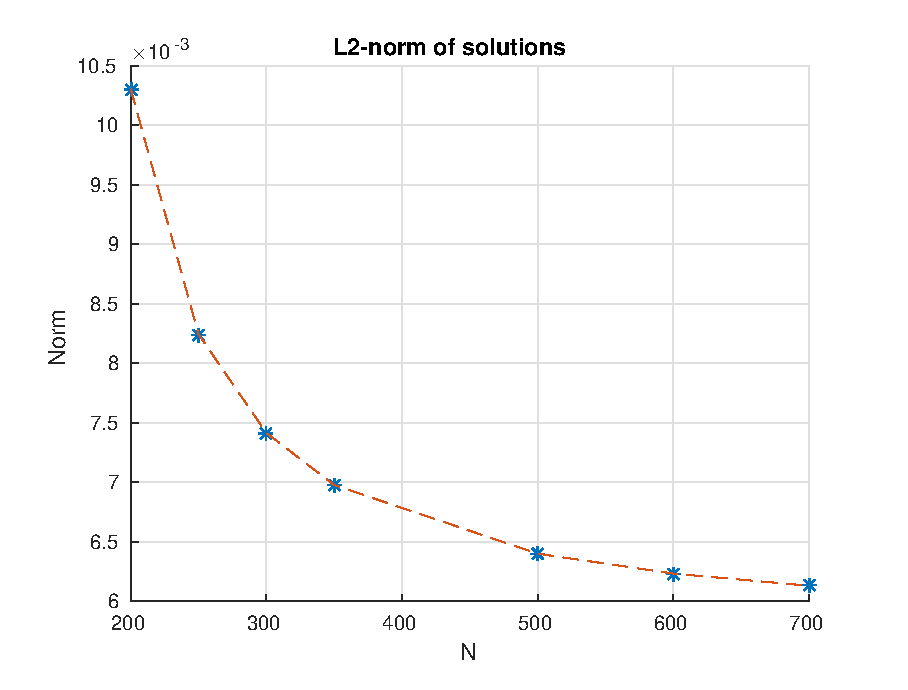
\includegraphics[scale=0.8]{figures/L2solutions}
    \caption{$\vectornorm{u_h}_{L^2(\Omega)}$ as a function of number of node points in each direction}
    \label{L2sol}
\end{figure} 

\begin{figure}
    \centering
    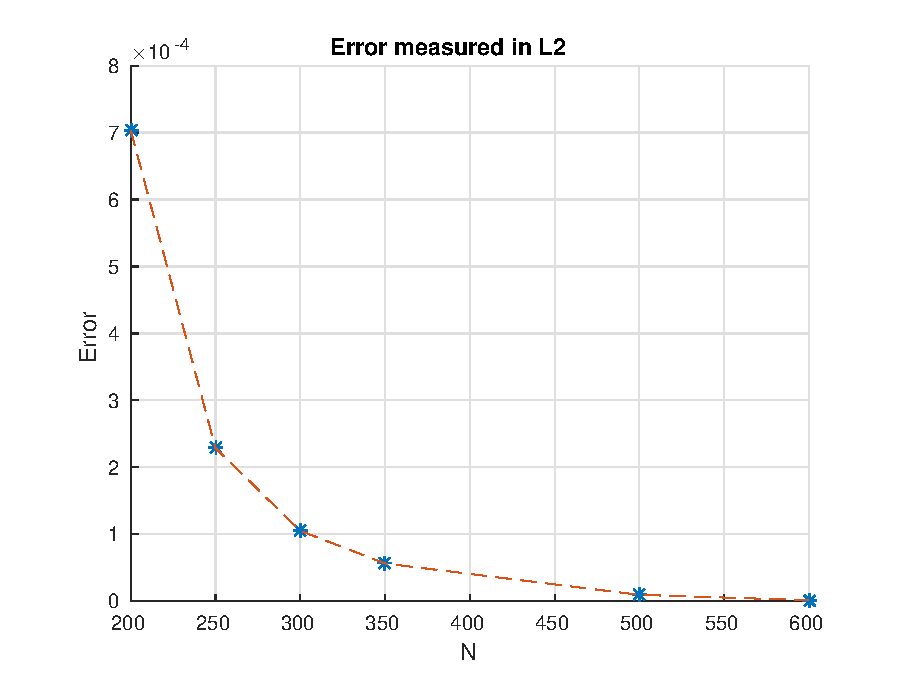
\includegraphics[scale=0.8]{figures/L2_error}
    \caption{$\vectornorm{u_{ref} - u_h}_{L^2(\Omega)}$ as a function of number of node points in each direction}
    \label{L2error}
\end{figure}


\end{document}

\documentclass[10pt,a4paper]{article}
\usepackage[latin1]{inputenc}
\usepackage{amsmath}
\usepackage{amsfonts}
\usepackage{amssymb}
\usepackage{mathtools}
\usepackage{bm}
\usepackage{standalone}
\usepackage{graphicx}
\usepackage{float}
% Use \bm{x} for vectors/matrices in bold AND italic

\begin{document}

\section*{Single Source In Unit Box}
\begin{figure}[H]
\centering
    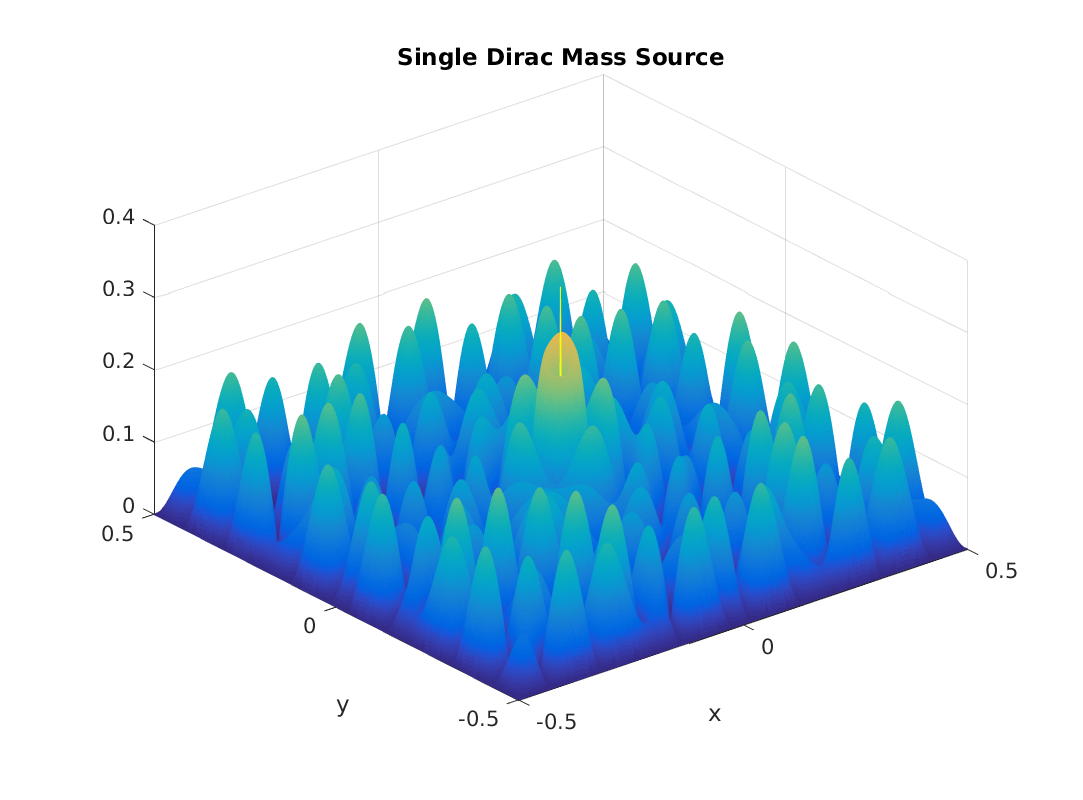
\includegraphics[width=0.9\textwidth]{figures/SingleSource_2D_1000.eps}
	\caption{A single source in unit box with Dirichlet boundary conditions.}
  \label{fig:severalSourcesDBC3D}
\end{figure}

\end{document}

\documentclass[10pt,a4paper]{article}
\usepackage[latin1]{inputenc}
\usepackage{amsmath}
\usepackage{amsfonts}
\usepackage{amssymb}
\begin{document}
\section*{Several Point Sources}
When solving the Helmholtz equation with several point sources, it is possible to see the interference between the different sources. In figure \ref{fig:severalSources} the two sources are located in (-0.25, -0.25) and (0.25, 0.25) and we can see the constructive interference in the origin.

\begin{figure}[h!]
\centering
    \includegraphics[width=0.9\textwidth]{figures/TwoSources_Dir3D.eps}
	\caption{Two point sources with Dirichlet boundary conditions plotted on the unit box.}
  \label{fig:severalSources}
\end{figure}

\end{document}

\documentclass[10pt,a4paper]{article}
\usepackage[latin1]{inputenc}
\usepackage{amsmath}
\usepackage{amsfonts}
\usepackage{amssymb}
\begin{document}
\section*{Solving Helmholtz For A House}
Insert final results and plots for the house here. This will typically be robin boundary conditions with complex wave numbers and one, maybe two sources.


\end{document}

\documentclass[10pt,a4paper]{article}
\usepackage[latin1]{inputenc}
\usepackage{amsmath}
\usepackage{amsfonts}
\usepackage{amssymb}
\usepackage{graphicx}
\usepackage{float}

\begin{document}

\begin{thebibliography}{}

\bibitem{Quarteroni}
Alfio Quarteroni, \emph{Numerical Models for Differential Problems}, 2nd Edition, 2014.

\bibitem{Project}
Ulrik Fjordholm, \emph{Programming project in TMA4220, part 2B:
Helmholtz' equation for electromagnetic waves} https://wiki.math.ntnu.no/$\_$media/tma4220/2015h/project2b.pdf, Nov 2015.

\bibitem{Helmholtz-Wave}
Tilo Arens, \emph{Helmholtz Equation - waveguides and scattering} https://people.maths.ox.ac.uk/trefethen/pdectb/helmholtz2.pdf, Nov 2015

\bibitem{ruppert}
J. Ruppert, \emph{A Delaunay Refinement Algorithm for Quality 2-Dimensional Mesh Generation}, 1995.

\bibitem{shewchuk}
J. Shewchuk, \emph{Delaunay Refinement Algorithms for Triangular Mesh Generation}, 2010.

\bibitem{miller}
G. Miller, S. Pav, N. Walkington, \emph{When and why Ruppert's algorithm works}, 2003


\end{thebibliography}

\end{document}

\end{document}

